\documentclass[crop=false,class=mitthesis,oneside,font=12pt]{standalone}
%----------------------------Preamble-------------------------------%
\usepackage{amsmath}
%\newcommand{\angstrom}{\textup{\AA}}
\usepackage{microtype}
\usepackage{graphicx}
\graphicspath{{./images/}}
%\usepackage{multirow}
\usepackage{rotating}
\usepackage{natbib}
\usepackage{url}
\usepackage{booktabs}
\usepackage{makecell}
\usepackage{graphicx, float}            % Graphics/Images.
\usepackage{pgfplots, tikz}             % Drawing/graphing tools.
\usetikzlibrary{
    calc,                   % Calculating right angles and more.
    angles,                 % Drawing angles within triangles.
    arrows.meta,            % Latex and Stealth arrows.
    quotes,                 % Adding labels to angles.
    positioning,            % Relative positioning of nodes.
    decorations.markings,   % Adding arrows in the middle of a line.
    patterns,
    arrows,
    shapes,
    shapes.geometric,
    cd,
    hobby,
    babel
}                                       % Libraries for tikz.
\pgfplotsset{compat=1.9}                % Version of pgfplots.
\usepackage[]{pdfpages}
% for line numbers comment the next two lines before final submission
\usepackage{lineno}
\linenumbers*[1]
% use fancyhdr, to enable page style stuff (below)
\usepackage{fancyhdr}
\setlength{\headheight}{15.2pt}
\renewcommand{\headrulewidth}{0pt}

\pagestyle{plain}
\usepackage{import}                     % Import external files.
\usepackage[subpreambles=false]{standalone}      % Complileable sub files.
\begin{document}
\chapter{Measurement techniques}
In this chapter, first, the historical background on the remote sensing and in-situ measurements of the IT system, with focus on optical remote sensing is given. Then, the details of the HiT\&MIS and spectral data collection process is described. After that, the reduction and analysis of the raw data is discussed. Finally, simple descriptions on other instruments and measurements used in this thesis is provided.
\label{chap:background}
\section{Overview}
%Balfour Stewart suggested existence of conducting layer of charged "air" in the upper atmosphere from small perturbations seen in magnetic measurements.
Measurements of the IT system is generally done using various plasma, neutral and optical measurement techniques. These include different radio measurement techniques, in-situ mass spectrometers, all-sky imagers, etc. Among radio techniques, the time profile of reflected or back-scattered radio waves are used to probe ionospheric parameters. Incoherent Scatter Radar (ISR) method works by sending high power radio wave at a fixed frequency into the ionosphere. The back-scattered profiles of the radio waves along with exact theoretical modeling is then used to infer density, velocity, temperature and spatial morphology of ionospheric plasma. Similarly, free electrons act as mirrors to radio waves below a critical frequency known as the plasma frequency, and so can act as a probe of ionospheric plasma using ionospheric sounding (ionosondes). Ionosondes operate by sending radio waves in a sweep of frequencies and then measuring the time profile of the reflected waves to infer electron densities. In addition to these radio techniques, GPS based radio transmitters can be used to probe the ionosphere by measuring the change in power and phase (brought about by the ionosphere) received at detectors on the ground to derive the line-of-sight integrated columnar electron density, also known as the Total Electron Content (TEC). 

Since the ionosondes requires small, portable radio wave generators and detectors, a network of ionosondes can be created (for example see \citet{giro}). While ISRs require large radio antennas, they can provide local spatial variations and be used to probe more plasma parameters (like temperatures and velocity) which ionospheric sounding can't probe. Similar to ionosonde, measurements form multiple network of GPS satellites allows for maps of TEC over large areas to be constructed, providing global morphology. 

Other measurement of the IT system include various in-situ charge particle detectors, mass spectrometers, etc., that can make direct measurements of plasma and neutral densities. Furthermore, optical measurements from ground and space can also be used to study the IT system if the processes involved in the observed emission is known. 

\subsection{Optical Remote Sensing}

Optical remote sensing of the IT system is a passive remote sensing technique as the airglow/auroral emissions act as proxies to IT processes. Early satellite based measurements of the upper atmosphere provided a wealth of information on prominent emission mechanisms and morphologies. For example, the limb scanning methods provided information on the altitude profiles of different airglow/auroral emissions and helped to better understand the processes leading to these emission. Satellite based optical measurements also provide large scale emission brightness morphologies at different latitude and longitudes, as well as, day/night variability. Red-line measurements from the Visible Airglow Experiment (VAE) which was on board the Atmospheric Explorer-C satellite, in conjunction with modeling was used to investigate the detailed photo-chemistry that give rise to the emission \citep{hays1978}. Using the green-line measurement from the same instrument, \cite{frederick1976} discussed processes that leading to the emission. In addition, \citet{orsini1977determination} discuss the photo-chemistry of the N$_2^+$ 427.8 nm vibrational band emission and  showed the height of its peak emission varies with season and magnetic activity. Further, sounding rocket experiments with multiple instruments can provide vertical profiles of auroral and airglow emission as well as in-situ plasma and/or neutral measurements near simultaneously. Such an approach is not only useful in getting the altitude profiles of emissions, but also to identify and constrain contribution of different sources that give rise to a particular emission.

While satellite-based optical measurements provide excellent spatial coverage, they lack temporal coverage at a given location. The ground-based instruments, on the other hand, lack the spatial coverage but can be used to observe temporal evolution of emission intensities. Ground-based photometric and/or spectrometric emission measurement also allow us to study IT system at different altitudes provided the emission sources are understood. Some of the information that can be inferred include the following:
\begin{itemize}
\item the column density of the emitting species has direct relationship with the emission intensity. So, if the optical instrument is photo-metrically calibrated the column density of emitting species can be retrieved.
\item Assuming thermal equilibrium between the surrounding and the emitting species, the line profile of an emission can be used to estimate the Doppler temperature and line of sight winds provided the line profile has enough resolution.
\item Provided the rotational structure of molecular emission is sensitive to the ambient gas temperature it can be used to estimate ambient gas temperature. Several band emissions that occur within the IT system, including the N$_2^+$ 427.8 nm, are sensitive to the ambient gas temperature.
\item The spatial and temporal changes in airgloe brightnesses can be used to study atmospheric dynamics caused by events like AGWs.
\item Simultaneous multi-spectral emission brightness measurements, can be used to study vertical propagation of atmospheric dynamics, such as during AGW events.
%In addition to the optical remote sensing 

%Various optical instruments have flown in rockets to investigate airglow and auroral emissions at different wavelength ranges
\end{itemize}

\section{HiT\&MIS}

The spectral data used in this thesis was collected using the HiT\&MIS instrument, which is a high-resolution ($\approx$ 0.02 nm at 630.0 nm) spectrograph, that can work on a round the clock basis \citep{hitmis}. HiT\&MIS follows a list of similar imagers that use a combination of slits, interference filters with the Echelle grating to select and image emission features of interest. These instruments include High Throughput Imaging Echelle Spectrograph (HiTIES, \cite{hities}), High-Resolution Imaging Spectrograph using Echelle grating (HIRISE, \cite{hirise}), Multi-wavelength Imaging Spectrograph using Echelle grating (MISE, \cite{mise}), Continuous High-resolution Instrument for Multiwavelength Echelle Spectroscopy (CHIMES, \cite{chimes}), etc. Each instrument was designed to image specific emissions at specific settings. For example, HiTIES was designed for night-time/twilight-time measurements, while CHIMES was designed for daytime measurements. These measurement constraints arise because requirements for daytime and night-time/twilight-time imaging are different. During the daytime, the solar background is orders of magnitude higher than the airglow/auroral emission signal, and thus high resolution is required to match with a solar reference spectrum so that the solar contribution can be subtract out. To obtain this, maximum dispersion of collected light is necessary which is achieved by using narrower slits as the throughput is not an issue during the day. During nighttime, the slit needs to be wide enough to have a enough throughput at reasonable temporal resolution. Thus, for round-the-clock measurement, the instrument needs to be designed to match both high-throughput and high-resolution requirements and be portable (Figure \ref{fig:hitmis_tripod}). This is where HiT\&MIS comes into consideration.

\begin{figure}[H]
	\centering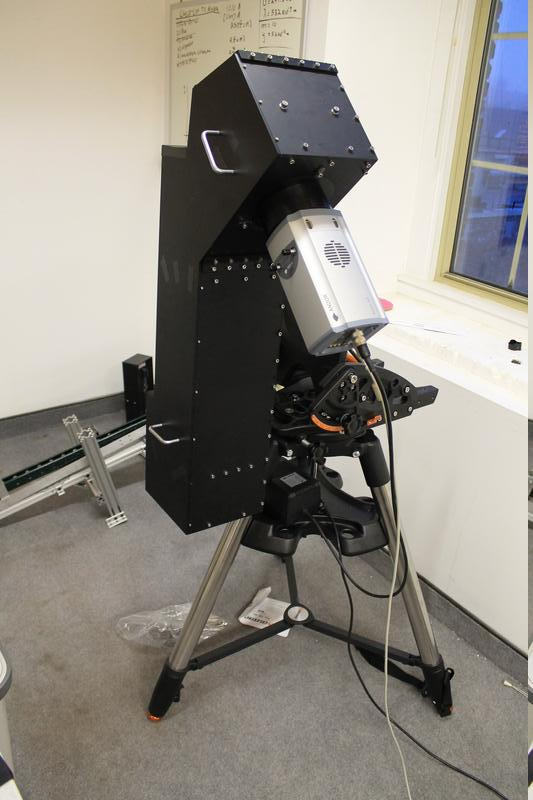
\includegraphics[width=25pc]{Hitmis_tripod_mount.JPG}
	\caption{HiT\&MIS mounted on a tripod. The portable design makes it versatile for campaign at different locations.}
	\label{fig:hitmis_tripod}
\end{figure}

The theoretical design of HiT\&MIS is schematically shown in Figure \ref{fig:hitmis}. It has a field of view of approximately 0.1$^\circ$ $\times$ 50$^\circ$ and a dispersion of about 0.02 nm/px in its current iteration.  Light enters through the four slits (numbered 1-4 in Figure \ref{fig:hitmis}), each of which is fitted with a narrow band filter (transmission properties listed in Figure \ref{fig:hitmis_tr}). There is also a mosaic of filter that is placed at the image plane. The light that has passed through the slits and the four entrance filters passes through a collimating lens (collimator/camera in Figure \ref{fig:hitmis}) and gets dispersed by the echelle grating in a near Littrow configuration. The diffracted light goes back into the same collimating lens that now acts as an imaging lens into a mosaic of interference filters (image plane filters in Figure \ref{fig:hitmis}). This combination of filters at the slits and the mosaic filters determines what spectral information is imaged. The image is then reflected through a folding mirror and refocused via a camera lens onto the CCD detector \citep{hitmis}.
\begin{figure}[H]
	\centering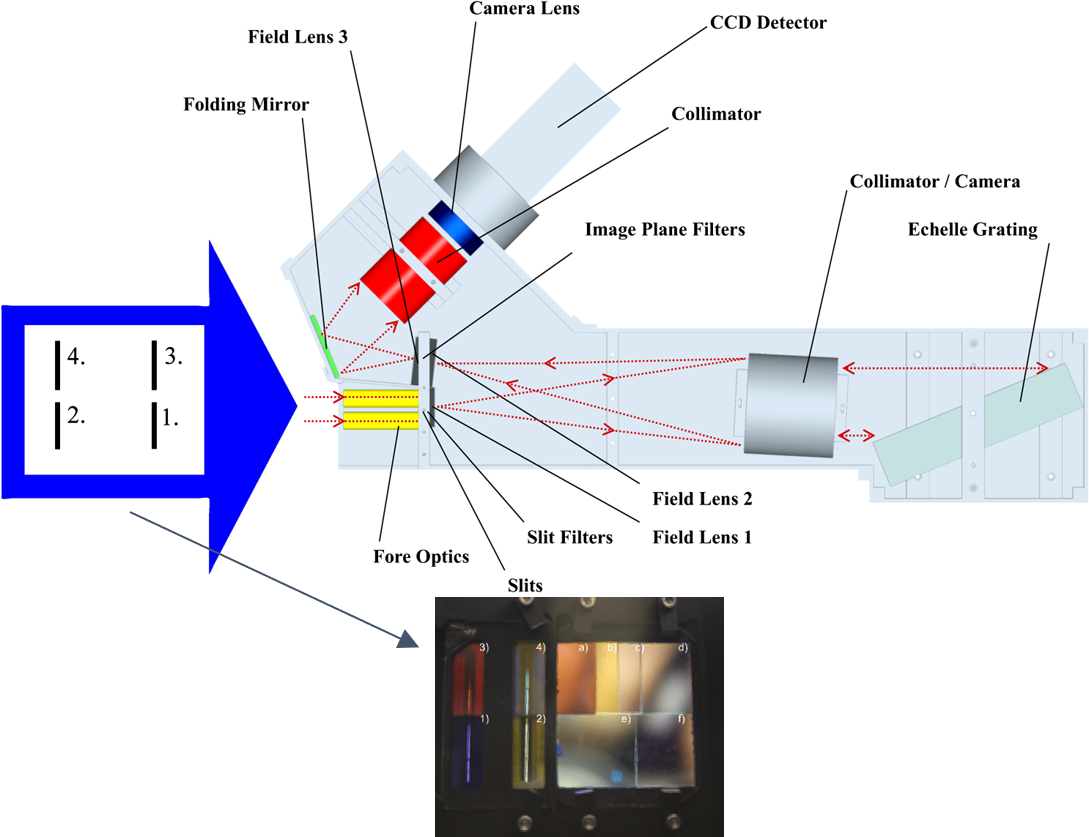
\includegraphics[width=25pc]{hitmis.png}
	\caption{Schematic diagram of the internal optics of the HiT\&MIS instrument. Adapted from \cite{hitmis}.}
	\label{fig:hitmis}
\end{figure}
%%%
\begin{figure}[H]
	\centering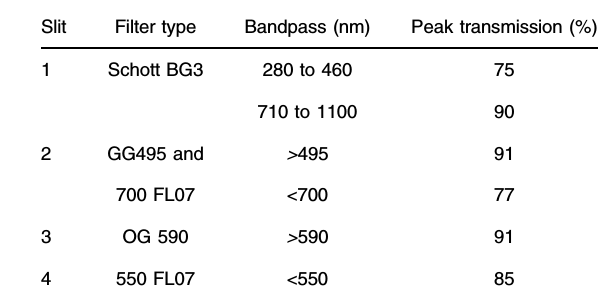
\includegraphics[width=25pc]{hitmis_tr.png}
	\caption{The transmission properties of the interference filters used in HiT\&MIS. Source: \cite{hitmis}.}
	\label{fig:hitmis_tr}
\end{figure}


HiT\&MIS has been developed to observe airglow and auroral emissions simultaneously at six selected wavelengths on a round-the-clock basis. The selected spectral features are: HI 656.3 nm, HI 486.1 nm, OI 557.7 nm, OI 630.0 nm, OI 777.4 nm and N$_2^+$ 427.8 nm. These emissions are key diagnostics to study the processes involved in airglow and aurora in detail. The six emission features that the HiT\&MIS instrument can observe are prominent emission features in the Earth’s upper atmosphere. The main excitation processes for the four emission features imaged by HiT\&MIS and used in this thesis are described in Table \ref{tbl:hm_emi}. 
%put tables of emission that hitmis can observe

%%%%%
%%%%
\section{HiT\&MIS Data Analysis}
%For this study, we used three spectral features observed by HiT\&MIS: blue line, green line and red line. 
\subsection{Characterization of CCD }
The spectral images were recorded using an Charged Coupled Device (CCD) camera cooled to -59$^\circ$ C. CCD cameras are semiconductor devices where photons that hit the CCD detector eject electron via the photo-electric effect and are excited to the conduction band where they can then be counted. To characterize the CCD, the bias frame and the dark frame were obtained by taking images with varying exposure times while the shutter was closed. The bias frame is a fixed pattern noise present in CCD images as a result of random quantum mechanical thermal fluctuations. Data counts (in Arbitrary Data Unit, ADU) on each pixel were then fitted to a linear equation to estimate the bias, B (in ADU)  and the dark frames, D (data units/s). The histograms for the bias and the dark frames are shown in Figure \ref{fig:biasdark}.  

\begin{figure}[H]
	\centering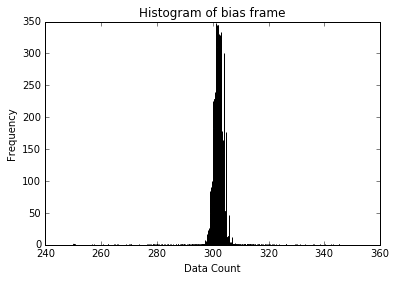
\includegraphics[width=30pc]{bias.png}
    \centering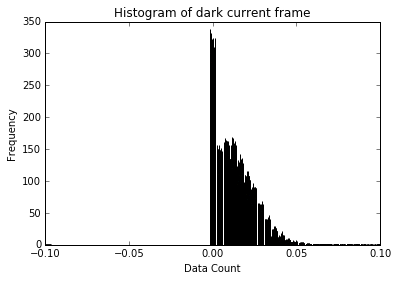
\includegraphics[width=30pc]{dark.png}
	\caption{Top: Histogram of the master bias, with a mean value of $\sim$ 300 ADU/pixel.  Bottom: Histogram of the master dark current, with mean value of 0.019 ADU px$^{-1}$ s$^{-1}$.}
	\label{fig:biasdark}
\end{figure}

\subsection{Emission line-center calibration}
\begin{figure}[H]
	\centering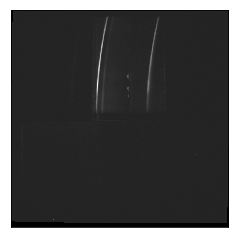
\includegraphics[width=20pc]{night_raw.png}
    \centering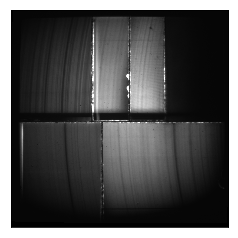
\includegraphics[width=20pc]{day_raw.png}
	\caption{Top: Sample night-time raw image from HiT\&MIS at 22:30 PM LT on June 22, 2015 with 60 s exposure. Bottom: Sample daytime raw image with 0.1 s exposure time at 17:30 PM LT on ths same day. Notice couple of spectral emission features are visible at night while absorbtion features are visible during the day.}
	\label{fig:raw_1}
\end{figure}
%
Figure \ref{fig:raw_1} shows an example of raw images collected by HiT\&MIS during day and night. While designing HiT\&MIS a ray trace simulation that was initially used to determine the different filters used instruments \citep{hitmis}. A set of filters were chosen to only let in lights around wavelength of interest and the emission features dispersed by the echelle was simulated (see Figure \ref{fig:hit_if}, top). Based on this ray trace result, mosaic of filters were chosen to select only the wavelength's of interest and the a ray trace was generated again using both entrance and the imaging mosaid filters (Figure \ref{fig:hit_if}, bottom). This final ray-trace can also be utilized to find the emission line center location on the CCD. During night, with enough cadence ($\sim$~60 s+) the red and the green lines are clearly visible on the detector (Figure \ref{fig:raw_1}, top). Similarly, during the day, the H$_\alpha$ and H$_\beta$ emissions show up as absorption features in the raw image (Figure \ref{fig:raw_1}, bottom). Thus, the ray trace results can be over-laid over the four emission feature location in the to validate the ray-trace simulation estimates as well as to to find emission line center locations. 
\begin{figure}[H]
	\centering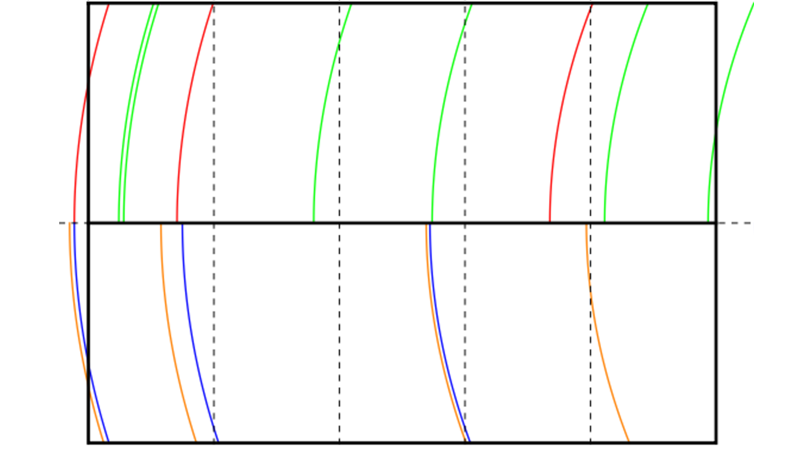
\includegraphics[width=30pc]{hit_i.png}
    \centering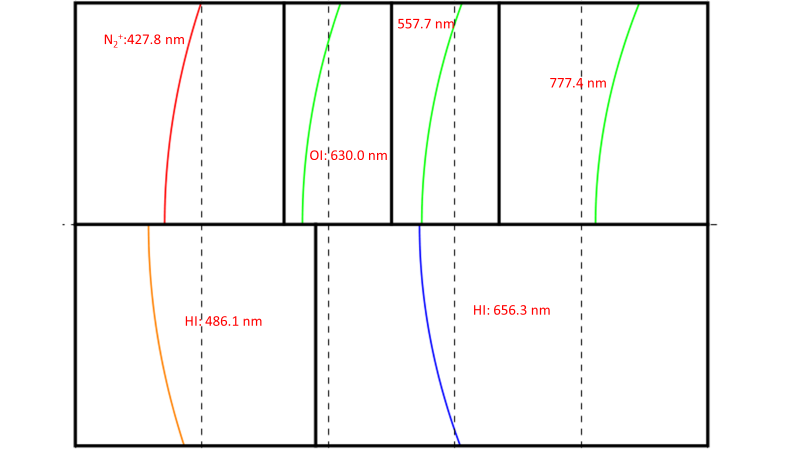
\includegraphics[width=30pc]{hit_f.png}
	\caption{Top: Ray trace modeling of emission lines from HiT\&MIS with only the entrance slits and filters. Bottom: Ray trace modeling of emission lines of interest from HiT\&MIS with the entrance slits and filters plus the image plane mosaic of filters. Notice that the overlapping lines disappear with the inclusion of mosaic of filters. Plot generated by Kuravi Hewawassam, UML}
	\label{fig:hit_if}
\end{figure}

The details of the the ray-trace simulation, similar to (but not the same) that used in \cite{hitmis} are now provided. To start, the following assumption were made to simplify the problem:
\begin{itemize}
\item all the filters were assumed to let in lights within $\pm$ 20 nm from central wavelength.
\item No estimates of the intensity was included, the light either came through or they didn't (binary scheme).
\item Only the wavelength of interest were let into the entrance filters.
\item The line from the center of the all the slits to the center of the Echelle are perpendicular.
\item The distance between the grating and the entrance slits and imaging mosaic filters are equal
\end{itemize}
%%
\begin{figure}[H]
	\centering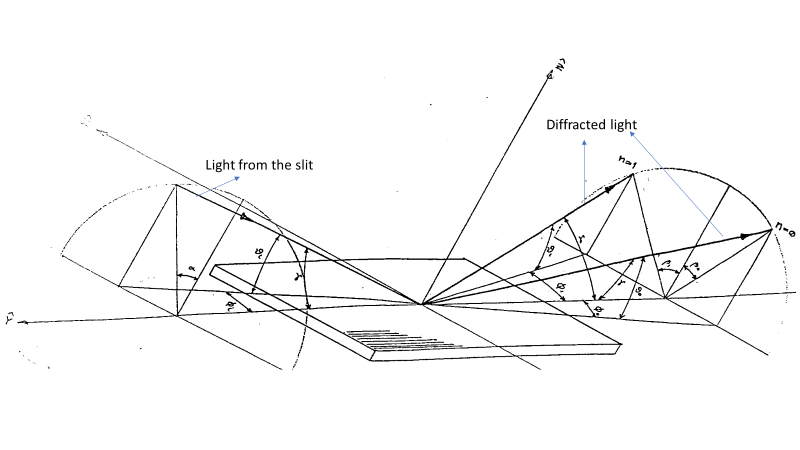
\includegraphics[width=35pc]{grating_stp.png}
	\caption{Geometry of spectral dispersion from to a grating. }
	\label{fig:grating}
\end{figure}

The light that entered through the entrance filters, now encountered the Echelle grating that disperses the light with the following grating equation:
%%
\begin{equation*}
\large
{n~\lambda~=d~sin\gamma~(sin\alpha + sin\beta_n)}
\end{equation*}
%%
\begin{equation}
\large
\implies~~\beta_n~=sin^{-1}\Big(\frac{n~\lambda~}{d~sin\gamma~}~-sin\alpha\Big).
\end{equation}
Here, d is the groove density of the grating, $\beta_n$ is the dispersion angle of the n$^{th}$ order at a particular ray entering through the slit at an angle $\gamma$ with respect to y-axis (see Figure \ref{fig:grating}). By measuring possible range of angles between the grating and the slit, the emissions at the imaging plane were simulated by taking following steps:
\begin{itemize}
\item Step1: Simulate all the emission lines passing through the slits, entrance filters and the grating (Figure \ref{fig:hit_if}, top). 
\item Step 2: Simulate the emission line that pass through the entrance slits that get dispersed by grating and select the mosaic of filters at the imaging plane that would only allow emissions of interest to pass through (Figure \ref{fig:hit_if}, bottom).
\end{itemize}
Once the ray-trace estimation location were made to match what was seen in the raw image (Figure \ref{fig:raw_line}), the region around the emission of interest are extracted for further analysis (Figure \ref{fig:cut_hm}). 
\begin{figure}[H]
	\centering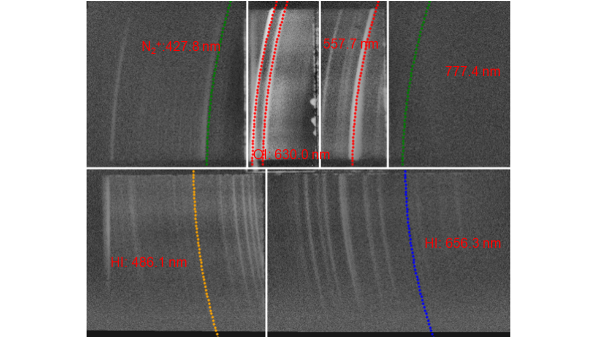
\includegraphics[width=32pc]{night_hm.png}
    \centering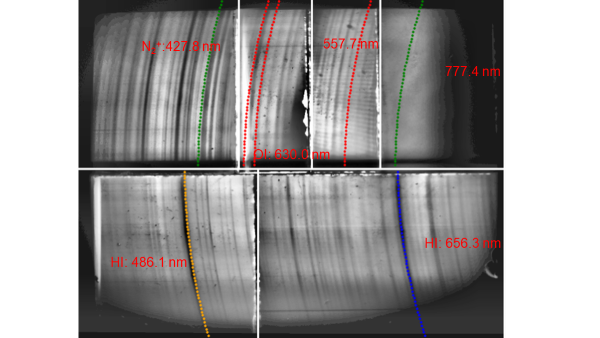
\includegraphics[width=32pc]{day_hm.png}
	\caption{Top: Sample night-time raw image from HiT\&MIS at 22:30 PM LT on June 22, 2015 with 60 s exposure. Overlaid lines are the ray trace estimate of the line center locations of the emission features shown in Figure . Bottom: Sample day-time raw image with 0.1s exposure. Notice that some of the emission feature at night-time image and absorption features and align with the ray-trace estimates.}
	\label{fig:raw_line}
\end{figure}

\begin{figure}[H]
	\centering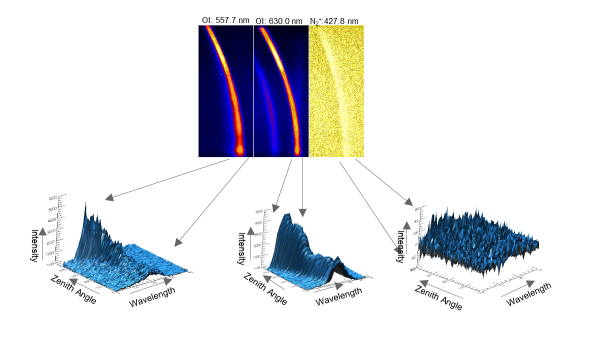
\includegraphics[width=35pc]{cut_hm.png}
	\caption{Top: Sample night-time raw image from HiT\&MIS at 22:30 PM LT on June 22, 2015 with 60 s exposure for the red line, green line and the N$2^+$ 427.8 nm. Bottom: Cut of background spectra extracted from Top.}
	\label{fig:cut_hm}
\end{figure}

\subsection{Photo-metric calibration}
HiT\&MIS creates spectral images of emissions as a function of wavelength and zenith angle (Figure \ref{fig:cut_hm}). For each spectral feature, the emission region over a narrow range of wavelength ($\approx$ $\pm$0.3 nm from the line center) was extracted from the image as mentioned in the last section. Then, the curvature in the measured spectrum as a function of zenith angle due to the slit geometry was corrected by transforming the cut-out spectral image such that the pixels with emission peaks are moved to the center. Finally, the baseline was estimated by averaging values on both side of the spectral feature and subtracted from the data, to obtain the signal, S. This gives the spectral signal (S), the background (B) and the readout noise (RN, standard deviation of the bias frame). The background subtracted spectra (un-calibrated) can now be represented as: $S \pm \sqrt{(S+B) + RN^2}$.  The analysis presented here applies only for night time data analysis. Possible daytime spectral imaging procedure for spectral imagers like HiT\&MIS is provided in Chapter 5.


\begin{figure}[H]
	\centering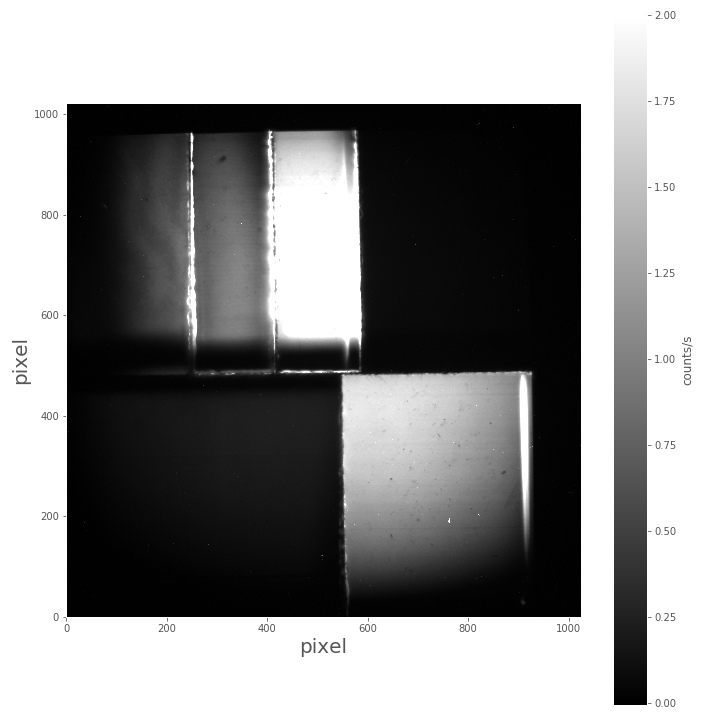
\includegraphics[width=30pc]{sen.png}
	\caption{Noise reduced master sensitivity image obtained by illuminating a calibrated lamp on to HiT\&MIS. As the output of the lamp as a function of the wavelength is known, this image was used to convert background subtracted data counts to photon counting units. }
	\label{fig:sen}
\end{figure}

A C-14 activated light source was used to calibrate the signal photo-metrically. This was done by illuminating HiT\&MIS with the calibration lamp for different increasing exposure times. These images were dark noise subtracted and averaged to get an the sensitivity of the instrument (in ADU per seconds) at each pixel (Figure \ref{fig:sen}). The output of the lamp is known and this was used to calibrate image data counts to physical units (in Raleigh $\rm {\AA}^{-1}$, see Figure \ref{fig:calib}, top). The calibrated spectra can then be averaged over different look direction bins (see Figure \ref{fig:calib}, bottom) to obtain a representative spectrum. Integrating the spectrum along the wavelength axis gives the line of sight brightness at different look directions. 
\begin{figure}[H]
	\centering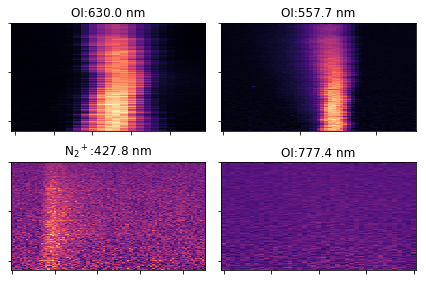
\includegraphics[width=30pc]{feature_img.png}
    \centering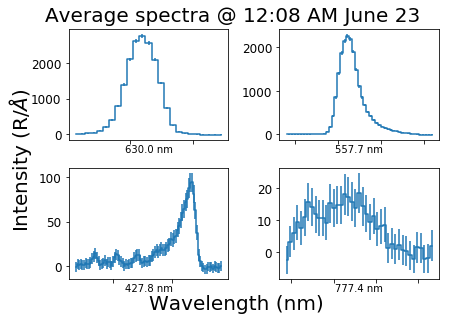
\includegraphics[width=30pc]{feature_spectra.png}
	\caption{Top: Curvature (due to slit geometry) straitened, noise reduced and photometrically calibrated spectra in red line, green line, blue line and OI 777.4 nm. Bottom: Same as top but averaged over look directions.}
	\label{fig:calib}
\end{figure}

\section{Other Measurement Techniques}
In addition to the optical remote sensing techniques, other techniques directly or indirectly used in this thesis are described in brief below. 

\subsection{Incoherent Scatter Radar (ISR)}
While ISR derived results are not used directly in this thesis, various other work cited in this thesis use ISR derived parameters extensively and thus a simplified picture of ISR is provided. Since the early 1960's, the Incoherent Scatter Radar has been the most used techniques to probe the ionosphere. This technique utilizes the incoherent scattering of the radio waves by ions and electrons in the ionosphere which occurs when the wavelength of the probing radio wave is smaller than the Debye length \citep{dougherty1963theory}. Above the Debye length (see Chapter 1) the charge particles are affected by each other such that the collective properties becomes coherent, both spatially and temporally. In general, the ISR measurements are not completely incoherent or coherent, however if the profiles of the incoherent back scatter are known they can be compared with theoretical models to obtain ionospheric parameters. 
%%%%
\begin{figure}[H]
	\centering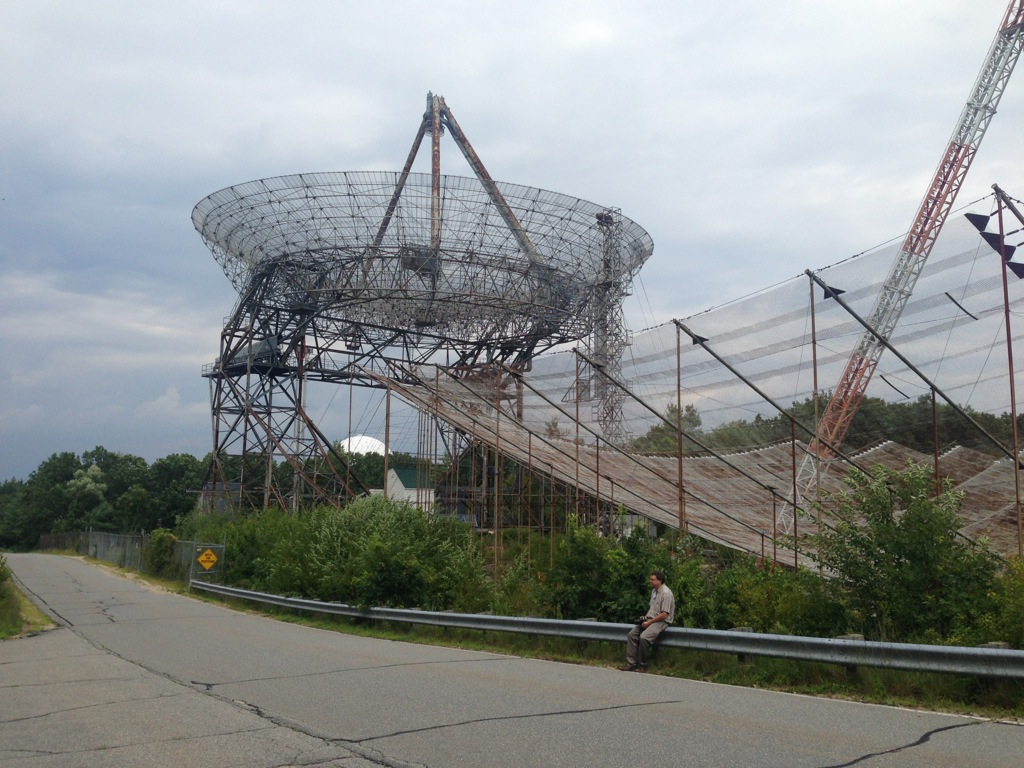
\includegraphics[width=30pc]{isr.jpg}
	\caption{ISR at MIT Haystack. Source: \url{http://blog.eiscat3d.org/2013/08/millstone-hill-incoherent-scatter-radar.html}}
	\label{fig:isr_a}
\end{figure}

The ISR technique works by sending high power radio waves at a fixed frequency, using a giant transmitter and antenna setup (see Figure \ref{fig:isr_a}). These radio-waves are then back-scattered by the electrons and ions incoherently which can be used to infer the their bulk properties. Since the ions are orders of magnitude heavier than the electrons, in frequency domain, the radio-waves back-scattered by the electrons and ions have completely different profiles (Figure \ref{fig:isr}), and hence can be used to probe both. In a simplified picture, the shift in frequency, the doppler width, and the area of the back-scattered profiles then are related to the line of sight velocity, the temperature and the plasma density, respectively. The radio-pulse sent to probe the ionosphere for ISR measurements, can be coded depending on the phenomenon to be studied and the altitude of focus.
\begin{figure}[H]
	\centering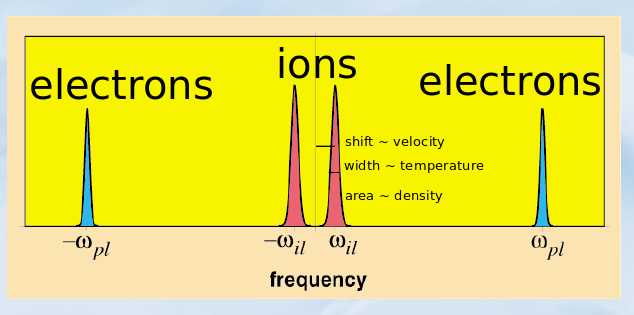
\includegraphics[width=30pc]{isr.png}
	\caption{ISR back scatter profile, and what different part of the profile signify. Adapted from \cite{anja}.}
	\label{fig:isr}
\end{figure}

\subsection{GPS-based Total Electron Content (TEC)}
Global Positioning System (GPS) uses multiple earth orbiting satellites ($\sim$ 32+) to mathematically triangulate a position on Earth. While GPS satellites are not geo-synchronous, if at least four satellites are visible at a given time, a receiver can accurately determine its location and velocity with the help an atomic clock (accuracy of 1 billionth of a second). As GPS technology uses radio signals to operate, the ionospheric plasma modulate the signal via radio waves plasma interaction. This modulation in both phase and amplitude of the signal is a proxy to the total electron content (TEC) the signal encounters along its path. With multiple receivers and GPS satellites, a map of the TEC can be made to study the effect of different phenomenon in the IT system. In this thesis, the Differential TEC( DTEC), which is the dynamic part of the TEC is used to study plasma waves in the IT system.
\begin{figure}[H]
	\centering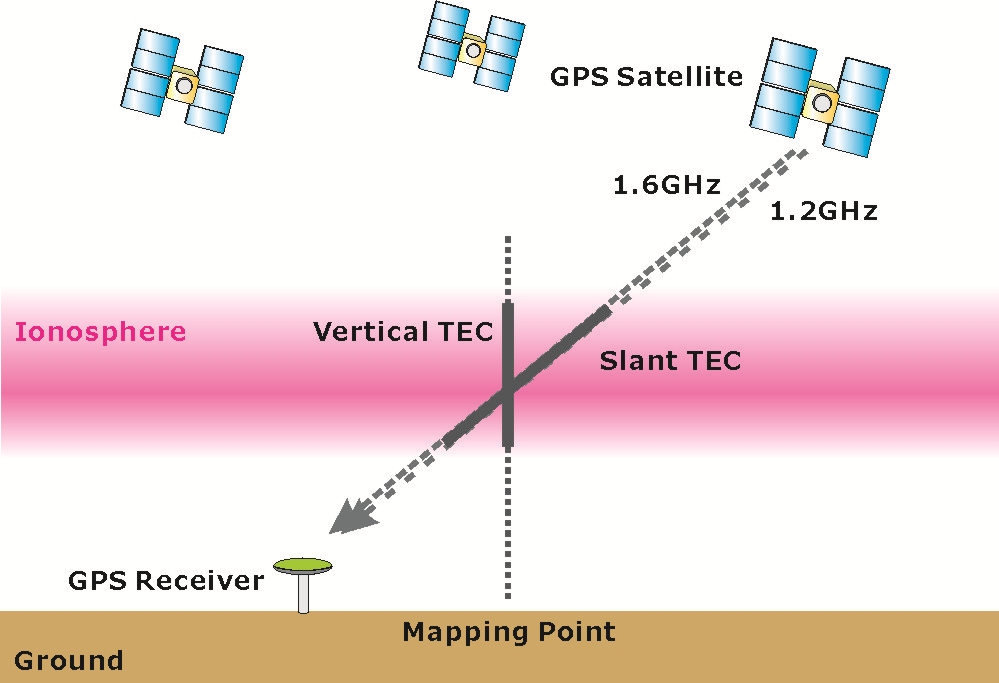
\includegraphics[width=30pc]{6-0.png}
	\caption{Schematic of GPS based TEC measurement. Source: \cite{tsugawa}.}
	\label{fig:gps}
\end{figure}

\subsection{Vertical Ionospheric Sounders (Ionosondes)}
Ionospheric sounding is another radio measurement technique to probe ionospheric plasma. It uses reflection of radio-waves above a critical frequency from the ionospheric plasma. Since the ionosphere is stratified into different plasma density peaks (Chapman layers), by probing in a range of radio frequencies, a vertical profile of the plasma density inferred. Thus, ionosonde broadcast radio waves at different frequencies which are then reflected only at certain frequencies from a particular ionospheric height which is then detected at ground (see Figure \ref{fig:digi_im} for the ionosonde setup). However, since the receiving times are different depending the altitude of reflection, an ionogram (like \ref{fig:digi_is}) is generated that can be converted into electron density profile.
\begin{figure}[H]
	\centering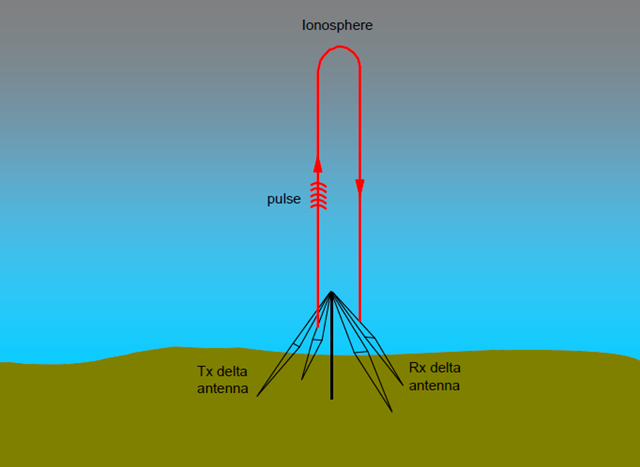
\includegraphics[width=30pc]{ionosonde.png}
	\caption{Schematic of a ionosonde system. Source: \cite{heather}.}
	\label{fig:digi_im}
\end{figure}

The index of refraction, n, for a radiation with frequency, f, incident on an electron distribution with density, N$_e$,  is given by:
\begin{equation*}
n^2~=~\Big(1~-~\frac{N_{e}~e^{2}}{4~\pi^{2}~\epsilon_{0}~m_{e}~f^{2}}\Big).
\end{equation*}
By defining a critical frequency, f$_c^2$ = $\frac{N_e~e^2}{4~\pi^{2}~\epsilon_{0}~m_{e}}$ , the index of refraction can be written as:
\begin{equation}
n^2~=1~-~\Bigg(\frac{f_c}{f}\Bigg)^2.
\end{equation}

From the equation \theequation, it follows that  the index of refraction for frequencies below the critical frequency (f $<$ f$_c$) is purely imaginary; at frequencies above the critical frequency (f $>$ f$_c$) it is purely real, and zero when the frequency of incident radio wave is equal to the critical frequency (f = f$_c$). This implies that at if the incident radiation is higher than the critical frequency of the medium, it penetrates the medium, where as below this frequency it is purely reflecting. Thus, if the ionosphere, with stratified ionization peaks (during the daytime), is probed with a sweep of frequency around the critical frequency a reflection profile as a function of frequency and reflection time (ionogram) can be created as shown in Figure \ref{fig:digi_s}. The ionogram can then be used to infer the electron density (by knowing f$_c$) profile as the time of return on to the detector measuring the reflection also gives information about the height were a particular frequency of radio wave was reflected from.
\begin{figure}[H]
	\centering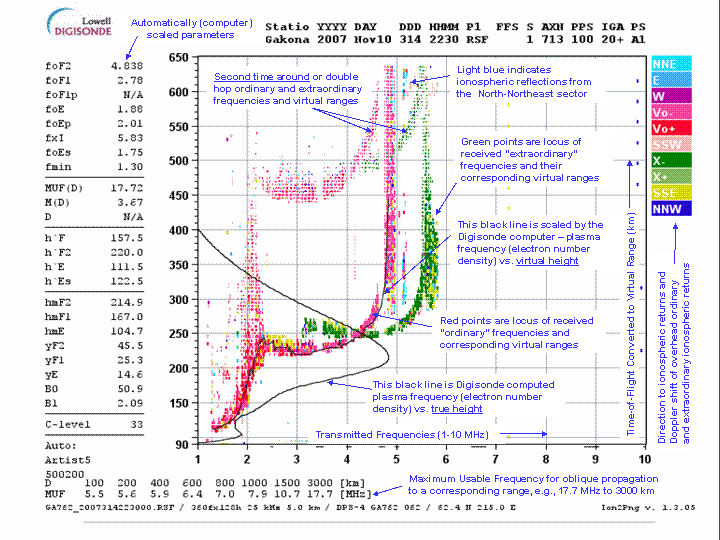
\includegraphics[width=30pc]{HAARP_ionogram.png}
	\caption{An example of a Ionogram. Source: \url{https://www.hfunderground.com/wiki/Ionosonde}}
	\label{fig:digi_s}
\end{figure}


\subsection{Magnetometers}
Magnetometers can be used to make precise measurement of the magnetic fields. While there are magnetometers that sense the magnetic field using other principles, only the fluxgate magnetometer is discussed herein. 

\begin{figure}[H]
	\centering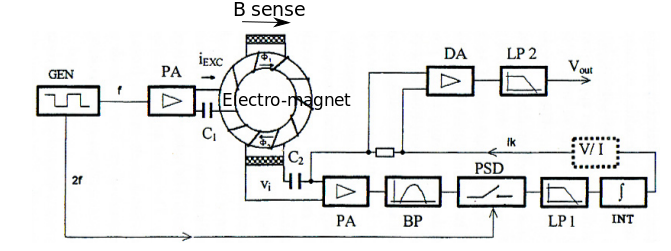
\includegraphics[width=30pc]{magnto.png}
	\caption{Schematic a single axis fluxgate magnetometer, with the sensing direction shown. Source: adapted from \cite{ripka2001magnetic}}
	\label{fig:magnemtr}
\end{figure}

Based on \citep{ripka2001magnetic}, a coil of wire with N turns and area A wrapped around a core with high relative magnetic permeability $\mu_r$; the magnetic constant $\mu_0$, a changing magnetic field B, with associated flux $\Phi$, will induce a voltage V such that,
\begin{equation*}
V~= \frac{d}{dt}\Phi~~=\frac{d}{dt}(N~A~\mu_{0}~\mu_{r}~B),
\end{equation*}using the Faraday's law. If B, A, and $\mu_r$ are functions of time, the voltage, V can be written as,
\begin{equation}
V=~N~A~\mu_{0}~\mu_{r}\frac{dB}{dt}+N~A~\mu_{0}~\mu_{r}~B\frac{dA}{dt}+N~A~\mu_{0}~B\frac{d\mu_{r}}{dt}
\end{equation}
From, equation \theequation, it is seen that modulating $\mu_r$ allows for the magnetic field B to be sensed. The discussion so far has been on a single axis magnetometer, where magnetic field component along one direction can be measured. However, changing the design of the magnetometer makes it possible to sense magnetic filed along three orthogonal axis. In this thesis, measurement of the Earth's magnetic field using AMPERE and the strength of ionospheric currents computed from these measurement is used.
\begin{figure}[H]
	\centering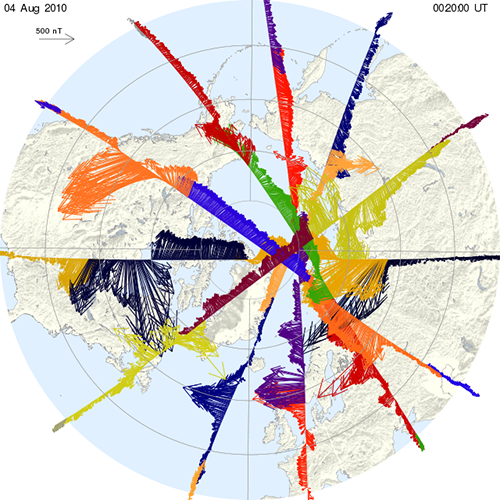
\includegraphics[width=30pc]{fac_s.png}
	\caption{Magnetic field in the polar region. The perturbations in these magnetic field can be used to infer the Field Aligned Current. Source: Johns Hopkins University Applied Physics Laboratory/AMPERE/R. J. Barnes}
	\label{fig:fac_s}
\end{figure}

\subsection{All Sky Imagers (ASIs)}
All sky imagers use narrow-band interference filters ($\sim \pm$ 20 nm from the central wavelength) and fish-eyed lens to image airglow/auroral emissions over the whole sky as seen from a particular location. This setup allows one to study the latitudinal/ longitudinal coupling of airglow/auroral emissions. Figure \ref{fig:asi_s} shows a typical all-sky imager setup. 
\begin{figure}[H]
	\centering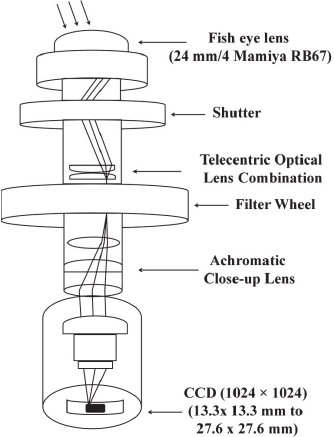
\includegraphics[width=30pc]{asi.jpg}
	\caption{Schematic example of a all-sky imager setup. Source: \cite{nade2012occurrence}}
	\label{fig:asi_s}
\end{figure}

ASI's give 2D auroral/airglow brightnesses; however, no spectral information can be obtained and thus there is a need to deal with contamination from nearby spectral features. This is in contrast with spectral imagers (like HiT\&MIS), where higher spectral resolution ($\sim$ 0.1 nm or less) allows for only the brightness feature of interest to be extracted, however only 1D airglow/auroral brightnesses (along the slit) can be observed.
\begin{figure}[H]
	\centering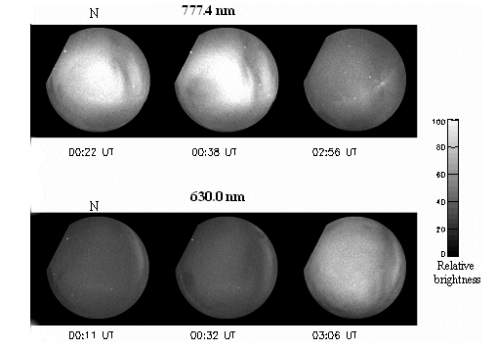
\includegraphics[width=30pc]{asi_mul.png}
	\caption{Near simultaneous raw ASI images in red line and OI: 777.4 nm at El Leoncito, Argentina on 30 May, 2003. From \cite{martinis2006imaging}  }
	\label{fig:asi_mult}
\end{figure}

Typically, ASI's use filter wheels to image multiple emissions of interest near simultaneously. Figure \ref{fig:asi_mult} shows near simultaneous raw ASI images at red line and OI: 777.4 nm line. Since the fish eye lens projects the features that are more spherical in 3D (due to the Earth's geometry) into a 2D image, the images near the edges are stretched. Thus, to project these emissions on to the map they are typically transformed based on the geographic location of the ASI and the peak height at which the emissions occur (see Figure \ref{fig:asi_urap}).

\begin{figure}[H]
	\centering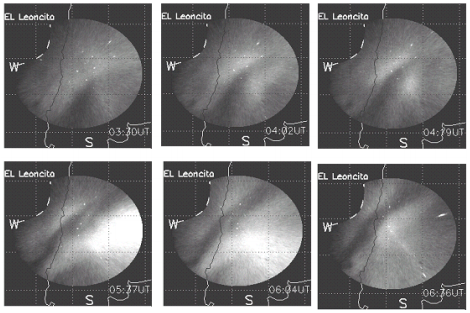
\includegraphics[width=30pc]{asi_urap.png}
	\caption{An example of all sky images in red line that has been transformed to be geographycally mapped. From \cite{martinis2006imaging} }
	\label{fig:asi_urap}
\end{figure}

\end{document}